% STATUS: ACTIVE | DERIVATION (2026-09-18) of the [2/2] Pade gain law in its coefficients (c_0, c_1, d_1, d_2), version A only:
%   four constant states, the gain COMPUTED from the law at the estimator's own height (no a slot). The a-slot writing
%   (version B of 0916_estb_11_two_versions.tex) needs a law autonomous in a_bar (a' a function of a_bar alone); [1/1] is
%   the widest such family (1/(1-a_bar) affine in g), [2/2] is not, so an a slot here could only alias the law value
%   (the R61 structure). Same nine-section reading copy as 0916_estb_11_two_versions.tex; the Jacobians are checked by
%   test_script/scratch/check_estb_22_jacobians.py (sympy, ALL PASS).
%   Controller: motion_control_law_formC_b.m flag pade22 (needs c0_state, gain_algebraic, amodel_fe, amodel_h; slots
%   5 = d_1, 7 = c_0, 8 = c_1, 9 = d_2; default off). Runner test_script/scratch/run_22_two_walls.m, figures plot_22_ladder.m.
%   Coordinate (2026-09-18): g = w_bar - w_bar_s = h_bar with w_bar_s the WALL SURFACE (plane 0), contact at g = 1.
%   Plane two-point (c_0, c_1, d_1, d_2) = (102/127, -229/127, -689/1016, -1/8), 1% on the band; cell band fit
%   (0.353, -0.571, 0.484, 0.058), 0.5% (0916_abar_gap_polynomial.tex sections 5-6). The old contact-height coordinate
%   (w_s = 1) is a linear change of basis that mixes c_0 with c_1 and d_2 with d_1, so the diagonal "half the spread" family
%   prior is NOT the same prior in the two bases (P/N arms differ between the 09-18 runs; T arms are bit-identical).
%   RESULT (ledger C59, canon 10 seeds, cell plant = data + [1/1] law tail, C60): the extra two constants buy the T arms'
%   residual (cell hold -0.006 vs [1/1] +0.017) and nothing for the wrong-seed arms -- one descent pins c_0 only, the
%   other three alias inside the band (plane N walks c_1/d_1/d_2 away from truth with the gain still right); the cell P
%   arm is NOT healthy (d_2 hits the 2*gap_floor guard in 10/10 seeds during 1.06-1.35 s), its mean must not be quoted.
% Compile: xelatex 0918_estb_22_versionA.tex

\documentclass[11pt,a4paper,fontset=none]{ctexart}
\usepackage[fleqn]{amsmath}
\usepackage{amssymb,bm}
\setlength{\mathindent}{0pt}
\usepackage{graphicx}
\usepackage{pdflscape}
\usepackage{geometry}
\geometry{margin=2.0cm}

\setlength{\parindent}{0pt}
\setlength{\parskip}{0.80em}
\linespread{1.08}
\setlength{\abovedisplayskip}{10pt}
\setlength{\belowdisplayskip}{10pt}

\newcommand{\ba}{\bar{a}}
\newcommand{\bw}{\bar{w}}
\newcommand{\dW}{\Delta\bw}
\newcommand{\ap}{\ba'}
\newcommand{\app}{\ba''}
\newcommand{\ah}{\hat{\ba}_w}
\newcommand{\ad}{\hat{\ba}_d}
\newcommand{\gh}{\hat g}
\newcommand{\gd}{\hat g_d}
\newcommand{\Nh}{\hat N}
\newcommand{\Dh}{\hat D}

\begin{document}

\section{Gain law}

(bars denote normalized quantities: lengths by $R$; $a_o := \Delta t/(\gamma_N R)$ [1/pN]; $\ba := a/a_{\mathrm{nom}}$;
$\bar f := a_o f$, so that $\ba\,\bar f = \dW$; $g := \bw - \bw_s = \bar h$, $\bw$ = particle centre along the wall normal,
$\bw_s$ = position of the wall surface on the same axis (plane: 0; cell: the visible surface), known, contact at $g = 1$;
$c_0, c_1, d_1, d_2$ = the $[2/2]$ coefficients, constants of the wall, fitted on the band $1.1 \le g \le 5.5$ and used there only;
$e_\theta = \theta - \hat\theta$)

\begin{align*}
N(g)   &:= g^{2} + c_1\,g + c_0, \qquad N'(g) = 2g + c_1 \\
D(g)   &:= g^{2} + d_1\,g + d_2, \qquad D'(g) = 2g + d_1 \\[4pt]
\ba(g;\, c_0, c_1, d_1, d_2) &= \frac{N(g)}{D(g)} \\[4pt]
1 - \ba &= \frac{(d_1 - c_1)\,g + (d_2 - c_0)}{D(g)} \\[4pt]
\ap(g)  &:= \frac{\partial\ba}{\partial\bw} = \frac{N'(g) - \ba\,D'(g)}{D(g)} \\[4pt]
\app(g) &:= \frac{\partial^{2}\ba}{\partial\bw^{2}} = \frac{2\,\bigl(1 - \ba\bigr) - 2\,\ap\,D'(g)}{D(g)}
\end{align*}

\begin{align*}
\Bigl(\frac{\partial\ba}{\partial c_0}\Bigr)_{g} &= \frac{1}{D(g)}, \qquad
\Bigl(\frac{\partial\ba}{\partial c_1}\Bigr)_{g} = \frac{g}{D(g)}, \qquad
\Bigl(\frac{\partial\ba}{\partial d_1}\Bigr)_{g} = -\,\frac{\ba\,g}{D(g)}, \qquad
\Bigl(\frac{\partial\ba}{\partial d_2}\Bigr)_{g} = -\,\frac{\ba}{D(g)} \\[6pt]
\Bigl(\frac{\partial\ap}{\partial c_0}\Bigr)_{g} &= -\,\frac{D'(g)}{D(g)^{2}}, \qquad
\Bigl(\frac{\partial\ap}{\partial c_1}\Bigr)_{g} = \frac{D(g) - g\,D'(g)}{D(g)^{2}} \\[6pt]
\Bigl(\frac{\partial\ap}{\partial d_1}\Bigr)_{g} &= \frac{\ba\,g\,D'(g)}{D(g)^{2}} - \frac{\ba}{D(g)} - \frac{\ap\,g}{D(g)}, \qquad
\Bigl(\frac{\partial\ap}{\partial d_2}\Bigr)_{g} = \frac{\ba\,D'(g)}{D(g)^{2}} - \frac{\ap}{D(g)} \\[6pt]
a_w &= a_o\,\ba_w
\end{align*}

\begin{align*}
\ba(1) &= \frac{1 + c_1 + c_0}{1 + d_1 + d_2}, \qquad
\ap(1) = \frac{(2 + c_1)(1 + d_1 + d_2) - (1 + c_1 + c_0)(2 + d_1)}{(1 + d_1 + d_2)^{2}}, \qquad
\lim_{g\to\infty} g\,\bigl(1 - \ba\bigr) = d_1 - c_1
\end{align*}

\section{True dynamics}

$\bigl(\delta\bw_j[k] := \delta\bw[k-d+j-1],\ j = 1,\dots,d+1,\ d = 2\bigr)$

\begin{align*}
\bw[k]           &= \bw_d[k] - \delta\bw_3[k] \\
\bw_d[k+1]       &= \bw_d[k] + \Delta\bw_d[k] \\
\ba_w[k]         &= \frac{N(\bw[k] - \bw_s)}{D(\bw[k] - \bw_s)} \\
\delta\bw_1[k+1] &= \delta\bw_2[k] \\
\delta\bw_2[k+1] &= \delta\bw_3[k] \\
\delta\bw_3[k+1] &= \lambda_c\,\delta\bw_3[k] - F_{dw}[k]\,e_{\ba_w}[k] - \varepsilon_w[k] \\
\dW[k]           &= \Delta\bw_d[k] + (1-\lambda_c)\,\delta\bw_3[k] + F_{dw}[k]\,e_{\ba_w}[k] + \varepsilon_w[k] \\
c_0[k+1]         &= c_0[k] \\
c_1[k+1]         &= c_1[k] \\
d_1[k+1]         &= d_1[k] \\
d_2[k+1]         &= d_2[k]
\end{align*}

\begin{align*}
F_{dw}[k]        &= \bar f_{dw}[k] + (1-\lambda_c)\sum_{i=1}^{d}\bar f_{dw}[k-i] \\
\varepsilon_w[k] &= \ba_w[k]\,\bar f_T[k] + (1-\lambda_c)\sum_{i=1}^{d}\ba_w[k-i]\,\bar f_T[k-i] - (1-\lambda_c)\,n_w[k]
\end{align*}

\section{Estimator A: four constant states, gain computed (no $a$ slot)}

($\gh[k] := \bw_d[k] - \delta\hat{\bw}_3[k] - \bw_s$; $\Nh := N(\gh;\,\hat c_0, \hat c_1)$, $\Dh := D(\gh;\,\hat d_1, \hat d_2)$;
controller slots: $5 = d_1$, $7 = c_0$, $8 = c_1$, $9 = d_2$)

\begin{align*}
\mathbf{x}_A &= \bigl[\,\delta\bw_1,\ \delta\bw_2,\ \delta\bw_3,\ c_0,\ c_1,\ d_1,\ d_2\,\bigr]^{\top}
\end{align*}

\begin{align*}
\ah[k]                 &= \frac{\Nh[k]}{\Dh[k]} \\
\delta\hat{\bw}_1[k+1] &= \delta\hat{\bw}_2[k] \\
\delta\hat{\bw}_2[k+1] &= \delta\hat{\bw}_3[k] \\
\delta\hat{\bw}_3[k+1] &= \lambda_c\,\delta\hat{\bw}_3[k] \\
\hat c_0[k+1]          &= \hat c_0[k] \\
\hat c_1[k+1]          &= \hat c_1[k] \\
\hat d_1[k+1]          &= \hat d_1[k] \\
\hat d_2[k+1]          &= \hat d_2[k]
\end{align*}

\section{Error dynamics A}

$\bigl(\mathbf{e}_A = [\,e_{\delta\bw_1},\ e_{\delta\bw_2},\ e_{\delta\bw_3},\ e_{c_0},\ e_{c_1},\ e_{d_1},\ e_{d_2}\,]^{\top}$, coefficients at the estimate$\bigr)$

\begin{align*}
e_{\ba_w}[k]         &= -\,\ap[k]\,e_{\delta\bw_3}[k]
                        + \frac{1}{\Dh[k]}\,e_{c_0}[k]
                        + \frac{\gh[k]}{\Dh[k]}\,e_{c_1}[k]
                        - \frac{\ah[k]\,\gh[k]}{\Dh[k]}\,e_{d_1}[k]
                        - \frac{\ah[k]}{\Dh[k]}\,e_{d_2}[k] \\[6pt]
e_{\delta\bw_1}[k+1] &= e_{\delta\bw_2}[k] \\
e_{\delta\bw_2}[k+1] &= e_{\delta\bw_3}[k] \\
e_{\delta\bw_3}[k+1] &= \bigl(\lambda_c + F_{dw}[k]\,\ap[k]\bigr)e_{\delta\bw_3}[k]
                        - F_{dw}[k]\,\frac{1}{\Dh[k]}\,e_{c_0}[k]
                        - F_{dw}[k]\,\frac{\gh[k]}{\Dh[k]}\,e_{c_1}[k] \\
                     &\quad + F_{dw}[k]\,\frac{\ah[k]\,\gh[k]}{\Dh[k]}\,e_{d_1}[k]
                        + F_{dw}[k]\,\frac{\ah[k]}{\Dh[k]}\,e_{d_2}[k] - \varepsilon_w[k] \\
e_{c_0}[k+1]         &= e_{c_0}[k] \\
e_{c_1}[k+1]         &= e_{c_1}[k] \\
e_{d_1}[k+1]         &= e_{d_1}[k] \\
e_{d_2}[k+1]         &= e_{d_2}[k]
\end{align*}

{\footnotesize\setlength{\arraycolsep}{2pt}
\begin{align*}
F_e^{A}[k] &= \begin{bmatrix}
0 & 1 & 0 & 0 & 0 & 0 & 0 \\
0 & 0 & 1 & 0 & 0 & 0 & 0 \\
0 & 0 & \lambda_c + F_{dw}[k]\,\ap[k]
      & -\dfrac{F_{dw}[k]}{\Dh[k]}
      & -\dfrac{F_{dw}[k]\,\gh[k]}{\Dh[k]}
      & \dfrac{F_{dw}[k]\,\ah[k]\,\gh[k]}{\Dh[k]}
      & \dfrac{F_{dw}[k]\,\ah[k]}{\Dh[k]} \\
0 & 0 & 0 & 1 & 0 & 0 & 0 \\
0 & 0 & 0 & 0 & 1 & 0 & 0 \\
0 & 0 & 0 & 0 & 0 & 1 & 0 \\
0 & 0 & 0 & 0 & 0 & 0 & 1
\end{bmatrix}
\end{align*}}

\section{Measurement}

$\bigl(\nabla_d\bw_d[k] := \bw_d[k] - \bw_d[k-d]$; $\gd[k] := \gh[k] - \nabla_d\bw_d[k]$;
$\Nh_d := N(\gd;\,\hat c_0, \hat c_1)$, $\Dh_d := D(\gd;\,\hat d_1, \hat d_2)\bigr)$

\begin{align*}
y_1[k]      &= \delta\bw_1[k] + n_w[k] \\
y_2[k]      &= \ba_w[k-d] + n_a[k] \\
\hat y_1[k] &= \delta\hat{\bw}_1[k] \\
\ad[k]      &= \frac{\Nh_d[k]}{\Dh_d[k]} \\
\hat y_2[k] &= \ad[k]
\end{align*}

{\footnotesize\setlength{\arraycolsep}{3pt}
\begin{align*}
H^{A}[k]    &= \begin{bmatrix} 1 & 0 & 0 & 0 & 0 & 0 & 0 \\[4pt]
               0 & 0 & -\ap(\gd[k])
                     & \dfrac{1}{\Dh_d[k]}
                     & \dfrac{\gd[k]}{\Dh_d[k]}
                     & -\dfrac{\ad[k]\,\gd[k]}{\Dh_d[k]}
                     & -\dfrac{\ad[k]}{\Dh_d[k]} \end{bmatrix}
\end{align*}}

\begin{align*}
\ap(\gd) &= \ap(\gh) - \nabla_d\bw_d\,\app(\gh) + \dots, \qquad
\Bigl(\frac{\partial\ba}{\partial\theta}\Bigr)_{\gd} = \Bigl(\frac{\partial\ba}{\partial\theta}\Bigr)_{\gh}
   - \nabla_d\bw_d\,\Bigl(\frac{\partial\ap}{\partial\theta}\Bigr)_{\gh} + \dots
\end{align*}

\begin{align*}
\mathbf{e}_y[k] &= H^{A}[k]\,\mathbf{e}^{-}[k] + \begin{bmatrix} n_w[k] \\ n_a[k] \end{bmatrix}
\end{align*}

\section{Noise}

\begin{align*}
Q^{A}[k]  &= Q_{33}[k]\,\mathbf{g}_A\,\mathbf{g}_A^{\top}, \qquad \mathbf{g}_A = \bigl[\,0,\ 0,\ -1,\ 0,\ 0,\ 0,\ 0\,\bigr]^{\top} \\
Q_{33}[k] &= \kappa_T\Bigl(\ah[k] + (1-\lambda_c)^{2}\bigl(\ah[k-1] + \ah[k-2]\bigr)\Bigr) + (1-\lambda_c)^{2}\sigma^{2}_{n_w},
\qquad \kappa_T = \frac{4k_BT\,a_o}{R} \\
R[k]      &= \mathrm{diag}\bigl(R_1,\ R_2[k]\bigr), \qquad R_1 = \frac{\sigma^{2}_{n}}{R^{2}}, \qquad
R_2[k] = 2a_{\mathrm{cov}}^{2}\,IF_{\mathrm{var}}\bigl(\ah[k]\bigr)\bigl(\ah[k] + \xi\bigr)^{2}
\end{align*}

\clearpage
\section{Observability}

($\Phi(k,k_0) := F_e[k-1]\cdots F_e[k_0]$, $\Phi(k_0,k_0) = I$; $N$ window length)

($O_w := R_w^{-1/2}\,[\,H[k_0]\Phi(k_0,k_0);\ \dots;\ H[k_0+N]\Phi(k_0+N,k_0)\,]$;
$O_w\,\mathbf{v}_i = \sigma_i\,\mathbf{u}_i$, $\sigma_1 \ge \dots \ge \sigma_7$)

\begin{align*}
\Delta\bw_d[k] = 0 \ \ \forall k,\ \delta\hat{\bw}_3 \to 0 \quad&\Longrightarrow\quad
F_{dw}[k] \to 0 \\
&\qquad\ \nabla_d\bw_d[k] = 0,\ \gh[k] = \gh\ \text{constant},\ \ah[k] = \ah\ \text{constant} \\
H^{A}[k]_{2,4:7} &\to \frac{1}{\Dh}\,\bigl[\,1,\ \gh,\ -\ah\,\gh,\ -\ah\,\bigr] \ \text{constant in } k \\
&\Longrightarrow\quad \bigl\{\mathbf{e} : e_{c_0} + \gh\,e_{c_1} - \ah\,\gh\,e_{d_1} - \ah\,e_{d_2} = 0\bigr\} \ \text{unobservable (dimension 3)}
\end{align*}

\begin{align*}
\text{heights } \bw_1,\dots,\bw_4:\qquad
\det\begin{bmatrix}
1 & g_1 & -\ba_1 g_1 & -\ba_1 \\
1 & g_2 & -\ba_2 g_2 & -\ba_2 \\
1 & g_3 & -\ba_3 g_3 & -\ba_3 \\
1 & g_4 & -\ba_4 g_4 & -\ba_4
\end{bmatrix} &\ne 0
\end{align*}

\section{Fixed height}

($\bw_d[k] = \bw_h$ for all $k$; $g_h := \bw_h - \bw_s$; $\ba_h := \ba(\bw_h)$ the plant's gain there; $r$ = the one number a single height pins)

\begin{align*}
\frac{g_h^{2} + c_1 g_h + c_0}{g_h^{2} + d_1 g_h + d_2} &= \ba_h
\quad\Longleftrightarrow\quad
c_0 + c_1\,g_h - \ba_h\,d_2 - \ba_h\,g_h\,d_1 = g_h^{2}\,(\ba_h - 1) \\[4pt]
r(\hat c_0, \hat c_1, \hat d_1, \hat d_2;\, \bw_h) &:= \hat c_0 + \hat c_1\,g_h - \ba_h\,\hat d_2 - \ba_h\,g_h\,\hat d_1 - g_h^{2}\,(\ba_h - 1)
\end{align*}

\begin{align*}
\text{four heights:}\qquad
\begin{bmatrix}
1 & g_1 & -\ba_1 g_1 & -\ba_1 \\
1 & g_2 & -\ba_2 g_2 & -\ba_2 \\
1 & g_3 & -\ba_3 g_3 & -\ba_3 \\
1 & g_4 & -\ba_4 g_4 & -\ba_4
\end{bmatrix}
\begin{bmatrix} c_0 \\ c_1 \\ d_1 \\ d_2 \end{bmatrix}
&= \begin{bmatrix} g_1^{2}(\ba_1 - 1) \\ g_2^{2}(\ba_2 - 1) \\ g_3^{2}(\ba_3 - 1) \\ g_4^{2}(\ba_4 - 1) \end{bmatrix}
\end{align*}

\section*{Seed and prior}

\begin{align*}
&\text{plane (two-point: } \ba(1) = 0,\ \ap(1) = 1,\ \app(1) = -\tfrac{327}{200},\ d_1 - c_1 = \tfrac{9}{8}\text{):} \\
&\qquad (c_0, c_1, d_1, d_2) = \bigl(\tfrac{102}{127},\ -\tfrac{229}{127},\ -\tfrac{689}{1016},\ -\tfrac{1}{8}\bigr) \\
&\text{cell (Fig.\ 11 band fit):} \\
&\qquad (c_0, c_1, d_1, d_2) = (0.353,\ -0.571,\ 0.484,\ 0.058) \\
&\text{(2026-09-16 contact-height coordinate } \bw_s' = \bw_s + 1:\ c_0' = c_0 + c_1 + 1,\ c_1' = c_1 + 2,\ d_1' = d_1 + 2,\ d_2' = d_2 + d_1 + 1) \\[4pt]
\hat c_0[0] &= c_{0,\mathrm{seed}}, \quad \hat c_1[0] = c_{1,\mathrm{seed}}, \quad \hat d_1[0] = d_{1,\mathrm{seed}}, \quad \hat d_2[0] = d_{2,\mathrm{seed}} \\
\ah[0] &= \frac{N(\bw[0] - \bw_s;\,\hat c_0[0], \hat c_1[0])}{D(\bw[0] - \bw_s;\,\hat d_1[0], \hat d_2[0])} \\
P[0]   &= \mathrm{diag}\bigl(P_{11}[0],\ P_{22}[0],\ P_{33}[0],\ \sigma_{c_0,0}^{2},\ \sigma_{c_1,0}^{2},\ \sigma_{d_1,0}^{2},\ \sigma_{d_2,0}^{2}\bigr) \\
&\text{wall family (half the plane--cell spread, in this basis):}\quad
 (\sigma_{c_0,0},\ \sigma_{c_1,0},\ \sigma_{d_1,0},\ \sigma_{d_2,0}) = (0.225,\ 0.616,\ 0.581,\ 0.092) \\
&\text{tight (own band fit):}\quad 0.05 \ \text{on all four} \\
&\text{denominator guard at the band floor:}\quad D(1.1) \ge 2\,g_{\mathrm{floor}}
\end{align*}

\begin{landscape}
\vspace*{\fill}
\noindent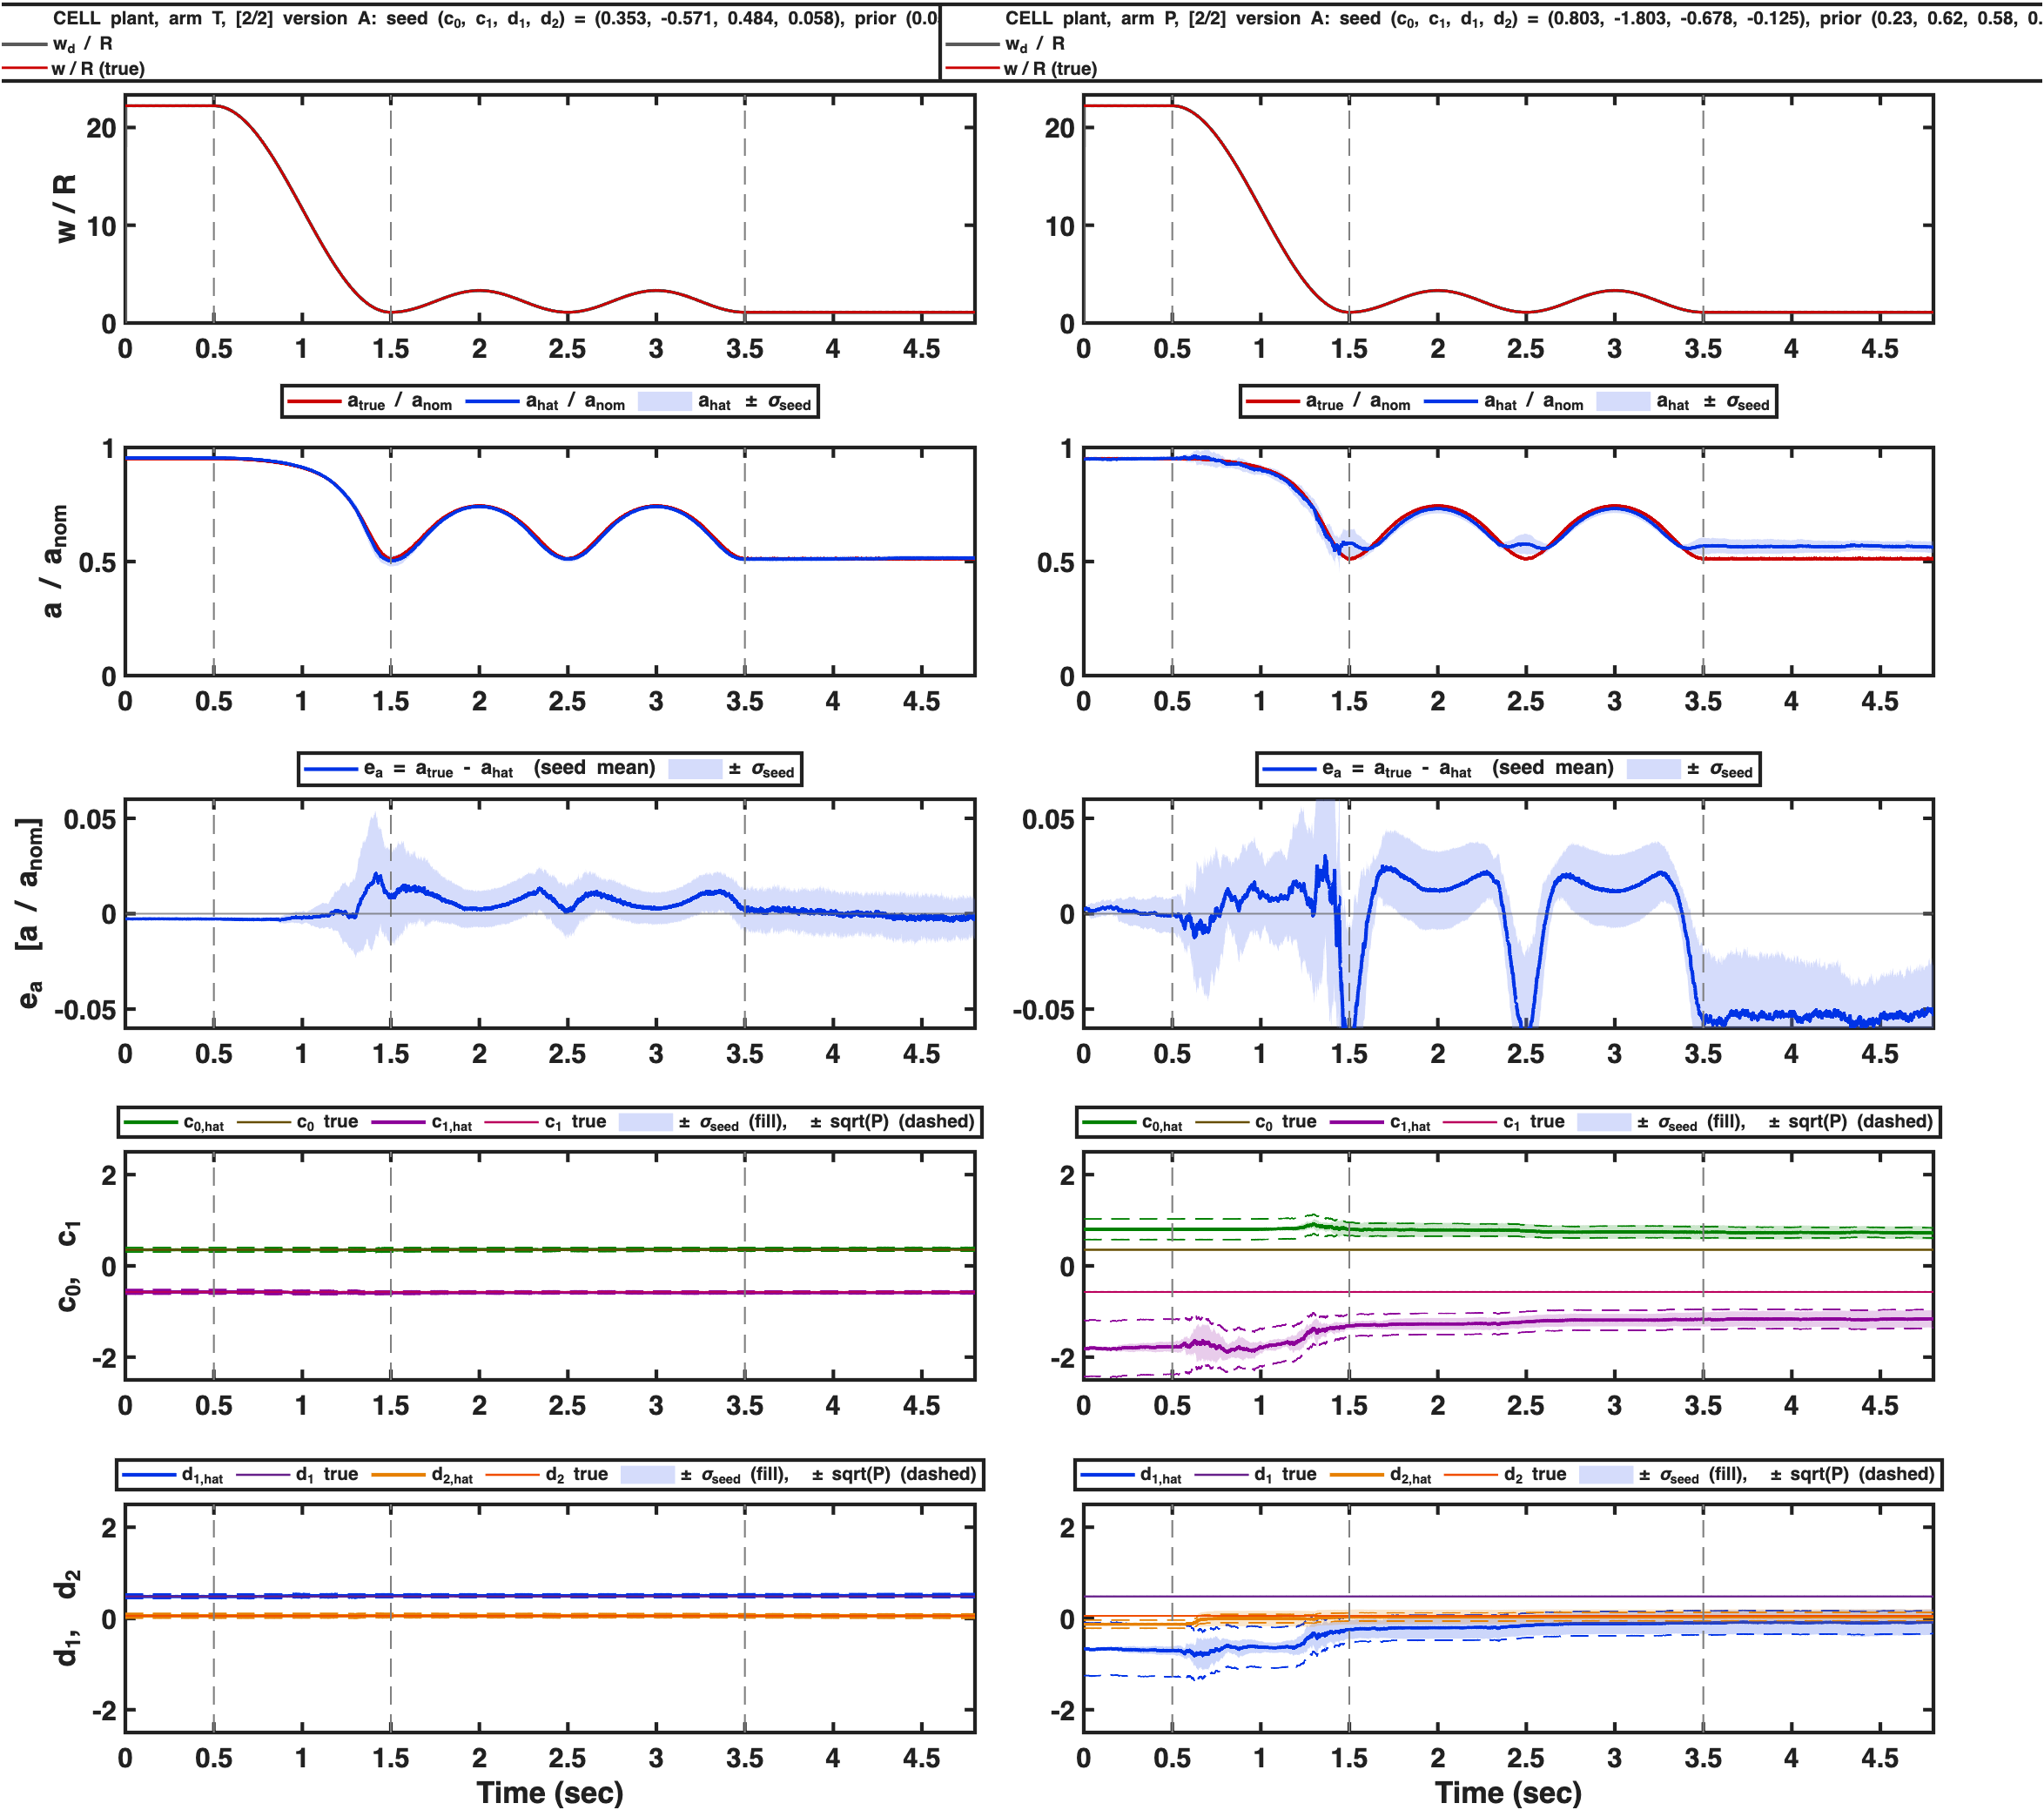
\includegraphics[height=0.95\textheight]{figures/ladder22_cell.png}
\vspace*{\fill}
\end{landscape}

\begin{landscape}
\vspace*{\fill}
\noindent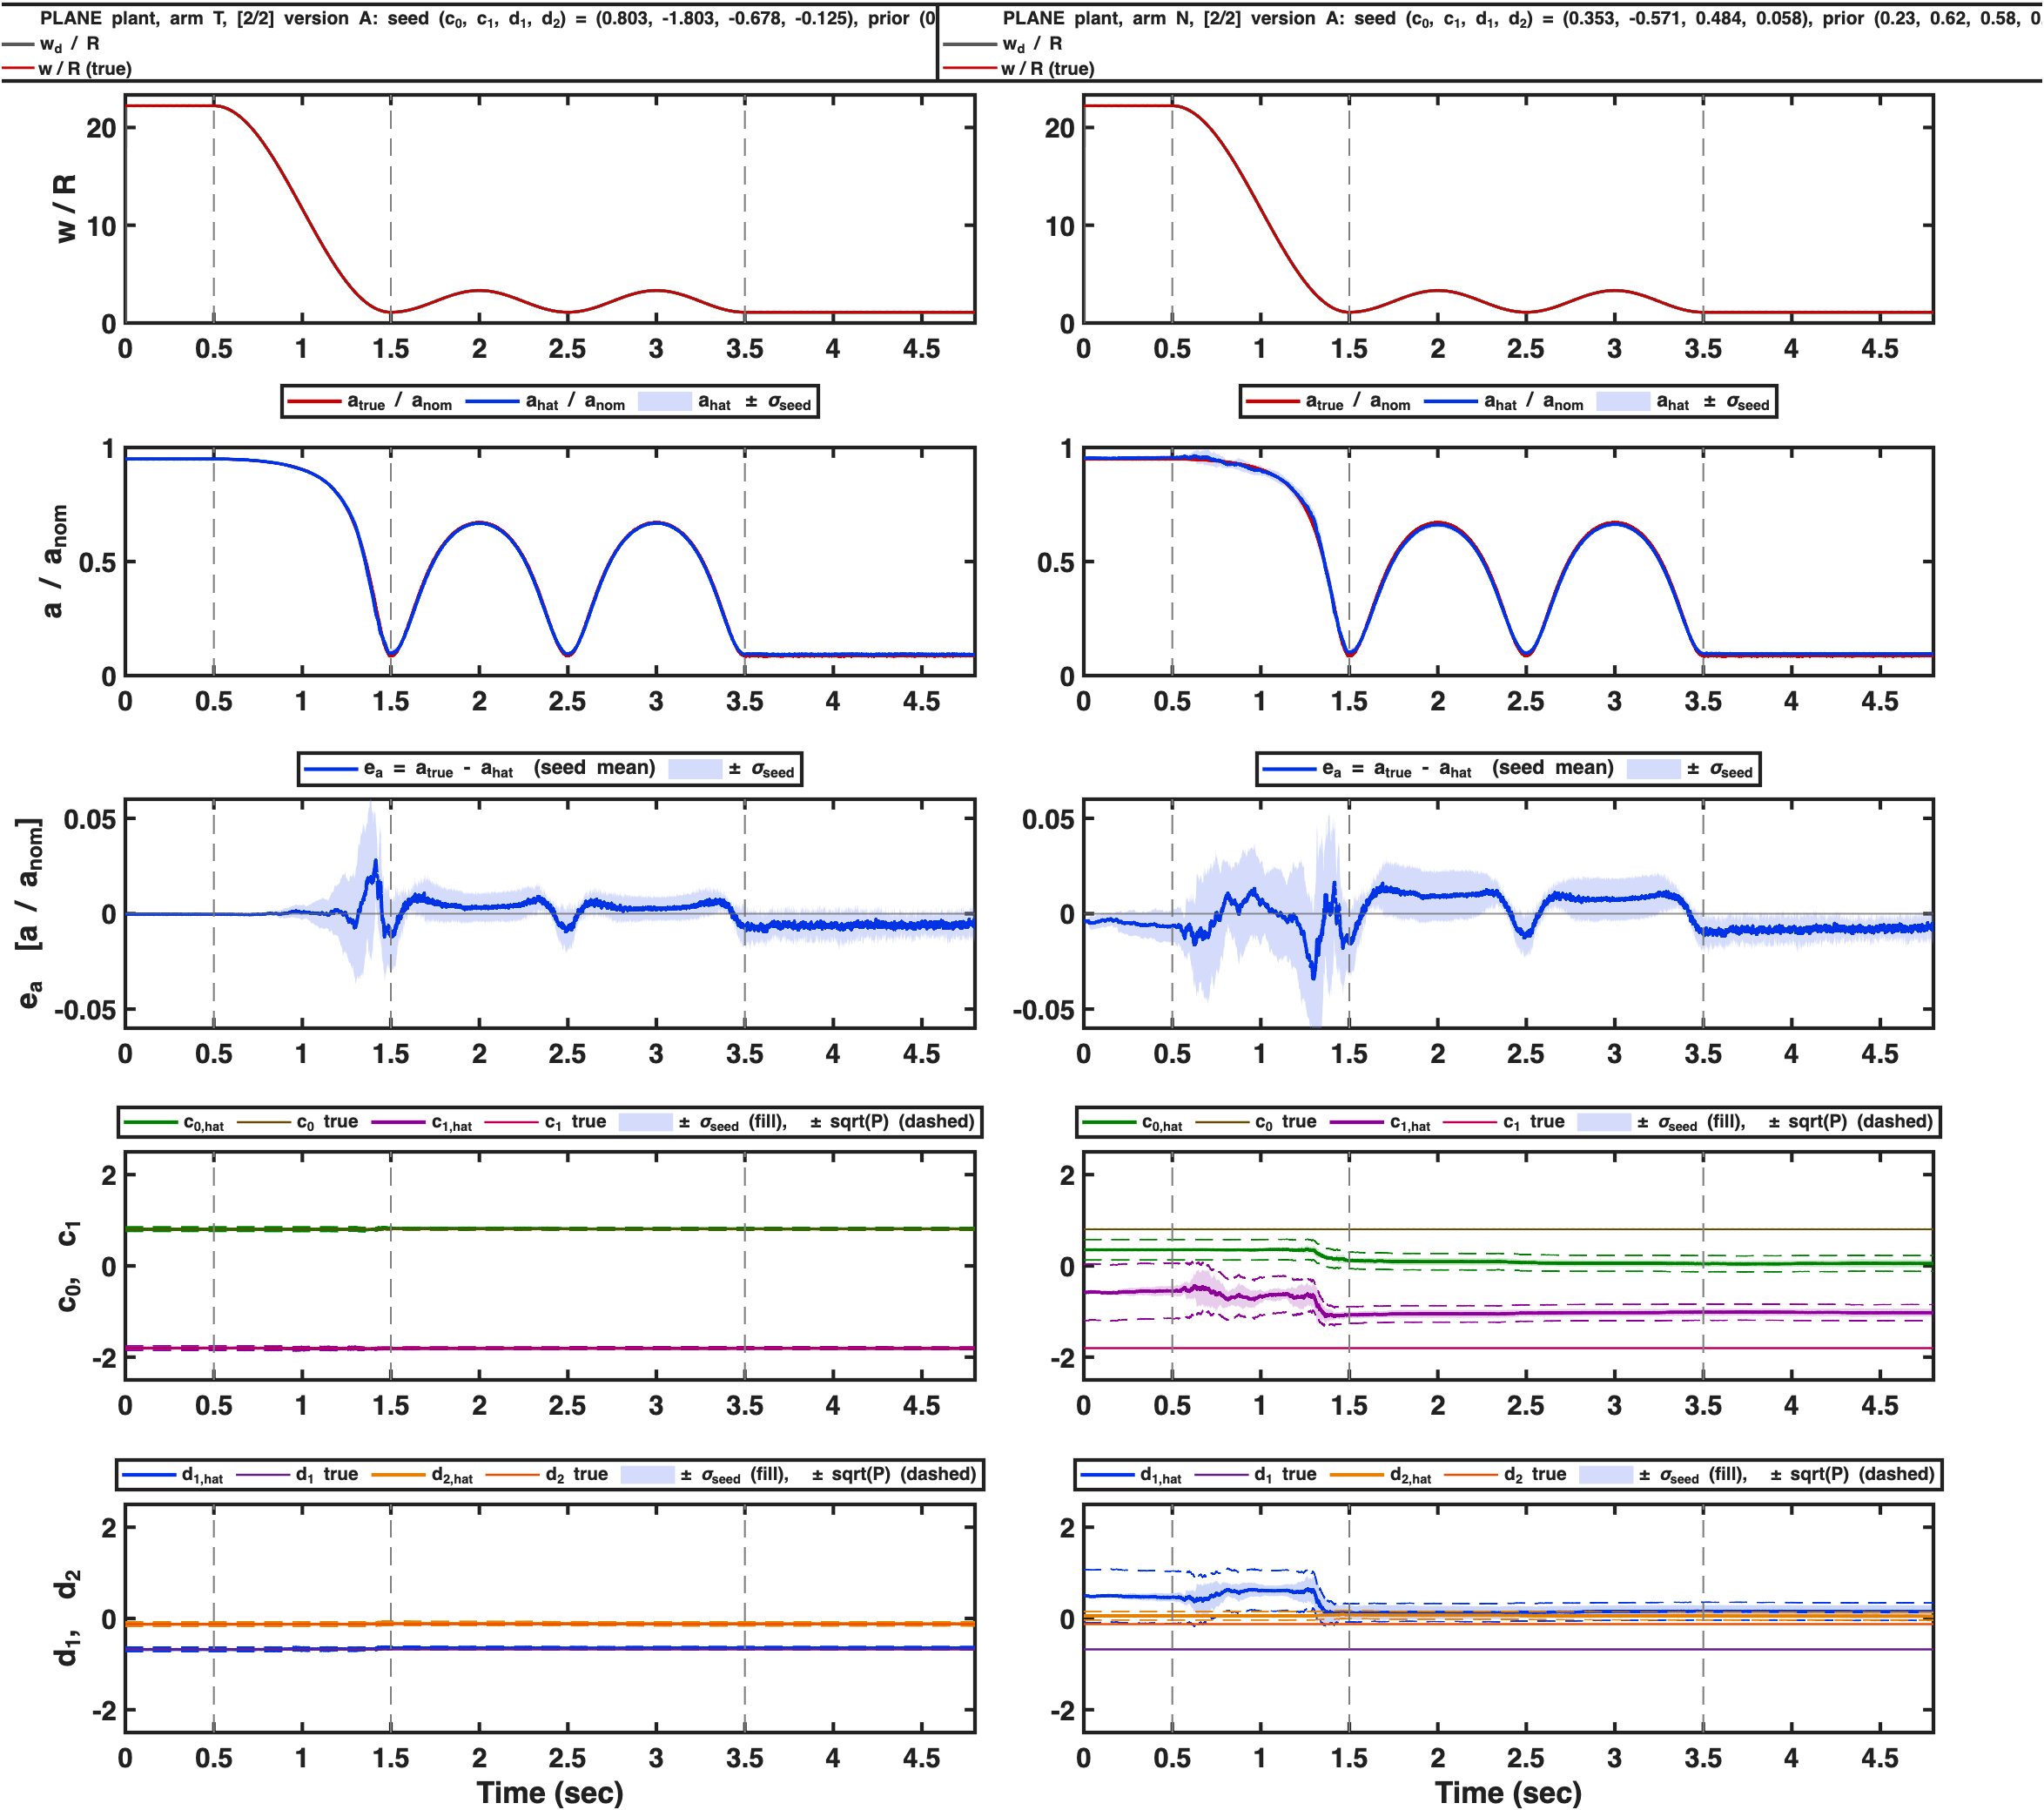
\includegraphics[height=0.95\textheight]{figures/ladder22_plane.png}
\vspace*{\fill}
\end{landscape}

\end{document}
